\documentclass[a4paper, 11pt]{article}
\usepackage{geometry}
\geometry{letterpaper, margin=1in}
\usepackage{amsmath}
\usepackage{amssymb}  Thank
\usepackage{amsthm}
\usepackage{ulem} 
\usepackage{graphicx}
\graphicspath{ {images/} }
\usepackage{tikz} 
\begin{document}
%Header-Make sure you update this information!!!!
\noindent
\large\textbf{Complex Analysis - MTH 483} \hfill \textbf{John Waczak} \\
\normalsize Day 7 \hfill  Date: \today \\

\subsection*{More Mobius examples}
Recall: $f(z) = \frac{z-1}{i(z+1)}$ takes the unit circle $|z|=1$ to the real line $y=0$ and $\hat{\mathbb{C}} = \mathbb{C} \cup \{\infty\}$ to the set $L = \{y=0\}\cup\{\infty\}$\\

\noindent \textbf{Riemann Sphere}
	\begin{figure}[!hbt]
		\centering
		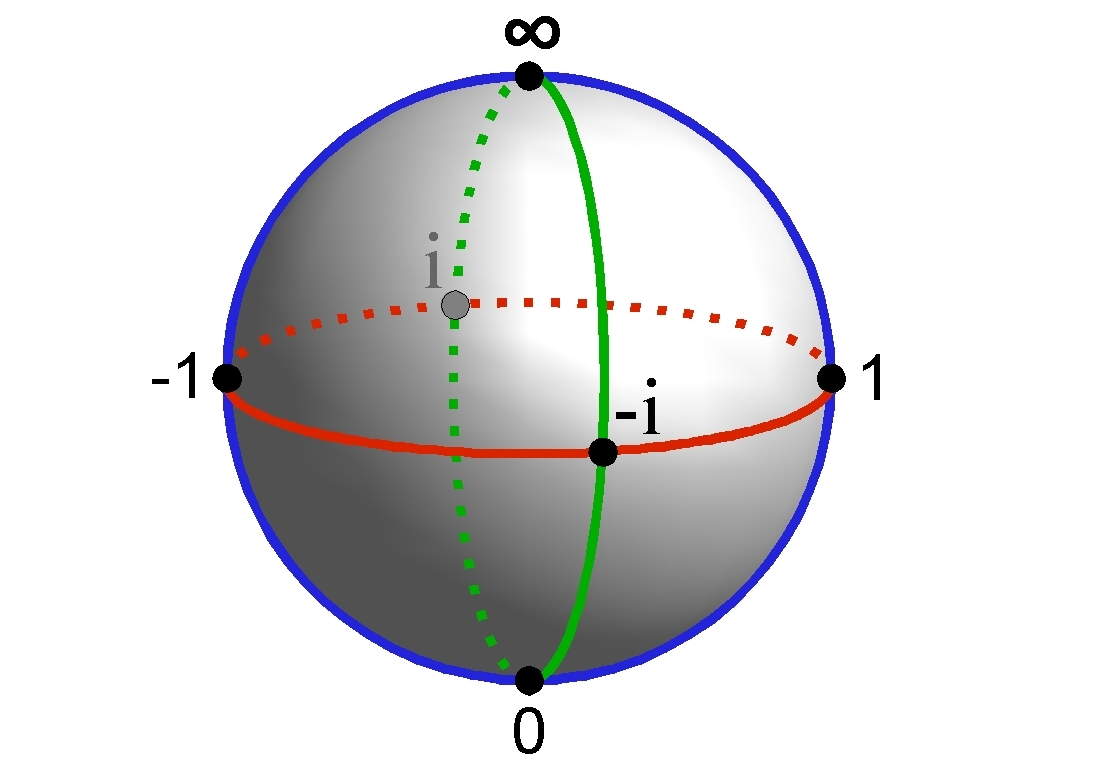
\includegraphics[width = 0.55\columnwidth]{riemannSphere}
	\end{figure}

\noindent\textit{Example:} Find the Mobius transformation that takes the circle $|z-1|=2$ to the circle $|z+(1+i)|=3$. \\

First the map $z\mapsto z-1$ translates $|z-1|=2$ to $|z|=2$. And, $z\mapsto \frac{3}{2}z$ takes $|z|=2$ to $|z|=3$. Finally, $z\mapsto z-(1+i)$ takes $|z|=3$ to $|z+(i+i)|=3$. Now we just compose:
	\begin{align*}
		f(z) &= \frac{3}{2}(z-1)-(1+i) \\
		|z-1|=2 &\mapsto |z+(1+i)|=3 
	\end{align*}

\noindent \textit{Example:} Find a Mobius transformation taking the circle $|z-1|=2$ to the line $x = 1$. \\

First recall that $f(z) = \frac{z-1}{i(z+1)}$ takes unit circle to real line... Thus $z\mapsto z-1$ takes $|z-1|=2$ to $|z|=2$. Now $z\mapsto z/2$ takes $|z|=2$ to $|z|=1$. Now $z \mapsto \frac{z-1}{i(z+1)}$ takes $|z|=1$ to $y=0$. Now we rotate by $\pi/2$ by multiplying by $i$ since $i=e^{i\pi/2}$. Thus $z\mapsto iz$ takes $y=0$ to $x=0$. Now $z\mapsto z+1$ takes $x=0$ to $x=1$. Therefore we have:
	\begin{align*}
		f(z) &= i\frac{\frac{1}{2}(z-1)-1}{i(\frac{1}{2}(z-1)+1)}+1\\
			&= \frac{\frac{1}{2}z-\frac{3}{2}}{\frac{1}{2}z+\frac{1}{2}}+1 \\ 
			&= \frac{z-3}{z+1}+1 \\ 
			&= \frac{z-3+z+1}{z+1} \\ 
			&= \frac{2z-2}{z+1}
	\end{align*}

\noindent Thus to go from circle to line just move circle to unit circle and then use $f(z)$. To go the other way just use the matrix inverse to find $f^{-1}(z)$. \\

\subsection*{Exponential sines and cosines}
\textbf{Define} $z\mapsto e^{z}$ (sometimes written $\exp(z)$) by the power series: 
	\begin{equation*}
		e^{z} = \sum_{n=0}^\infty \frac{z^n}{n!} \quad \forall z\in\mathbb{C}
	\end{equation*}

A few facts to report:
	\begin{itemize}
		\item This power series converges absolutely $\forall z \in \mathbb{C}$ and defines a holomorphic function $\mathbb{C}\rightarrow \mathbb{C}$.
		
		\item In terms of $z=x+iy$ we will see $e^{x+iy} = e^x(\cos(y)+i\sin(y))$. It would be \textit{cheating} to use this as a definition (as in the book)...
		
		\item $e^{z+w}=e^ze^w$ 
		
		\item $|e^{x+iy}| = e^x$ 
		
		\item $e^0 = 1$ 
		
		\item $|e^{iy}|=1$ 
		
		\item $\frac{1}{e^z} = e^{-z}$ 
		
		\item $e^z \neq 0$ 
		
		\item $e^{z+2\pi i} = e^z$ 
	
	\end{itemize}

Recall the binomial theorem: 
	\begin{align*}
		(z+w)^n &= \sum_{j=0}^n (n,j)z^jw^{n-j} \\ 
		(n,j) &= \frac{n!}{j!(n-j)!} \\ 
		\text{ex: } \quad (z+w)^2 &= z^2+zw+w^2 \\ 
			(z+w)^3 &= z^3 + 3z^2w + 3zw^2 + w^3 
	\end{align*}


\noindent Now, 
	\begin{align*}
		e^{z+w} &= \sum_{n=0}^\infty \frac{1}{n!}(z+w)^n \\
			&= \sum_{n=0}^\infty \frac{1}{n!}\sum_{j=0}^n (n,j)z^jw^{n-j} \\
			&= \sum_{n=0}^\infty\sum_{j=0}^n \frac{z^jw^{n-j}}{j!(n-j)!} \\
			&= \sum_{j=0}^\infty \sum_{n=j}^{\infty} \frac{z^jw^{n-j}}{j!(n-j)!} \\ 
			&= \sum_{j=0}^\infty \frac{z^j}{j!} \sum_{n=j}^{\infty} \frac{w^{n-j}}{(n-j)!} \\
		 \text{let } m=n-j \quad &= \sum_{j=0}^\infty \frac{z^j}{j!}\sum_{m=0}^\infty \frac{w^m}{m!} \\ 
		 	&= \Bigg(\sum_{j=0}^\infty \frac{z^j}{j!}\Bigg)\Bigg(\sum_{m=0}^\infty \frac{z^m}{m!}\Bigg) \\ 
	\end{align*}

Now we can define $cos$ and $sin$ in terms of power series:
	\begin{center}
	\centering
	\begin{enumerate}
		\item $\cos z = \frac{e^{iz}+e^{-iz}}{2}$ 
		\item $\sin z = \frac{e^{iz}-e^{-iz}}{2i}$
		\item $\cos z = \sum_{n=0}^\infty \frac{(-1)^n}{(2n)!}z^{2n}$
		\item $\sin z = \sum_{n=0}^\infty \frac{(-1)^{n+1}}{(2n+1)!}z^{2n+1}$
	\end{enumerate}
	\end{center}





\end{document}































